\documentclass[output=paper]{langsci/langscibook}
\ChapterDOI{10.5281/zenodo.1407007}

\title{The Haitian Creole copula and types of predication: A Word-and-Pattern account}
\shorttitlerunninghead{The Haitian Creole copula and types of predication}

\author{Alain Kihm   \affiliation{CNRS, Université Paris-Diderot} }

\abstract{ Haitian Creole is a French-based creole\il{Creole} language spoken by about 10 millions people in Haiti. In Haitian Creole the copula consists in the two forms \emph{se} and \emph{ye} and it may not be expressed. The present paper argues that, despite claims to the contrary, the Haitian Creole copula is a verbal lexeme realized through two overt suppletive stems and a phonologically null stem. Selecting one stem or the other does not depend on inherent and/or contextual inflectional features as in English \emph{am} vs. \emph{is} vs. \emph{was} vs. \emph{were}, but on the syntax and semantics of the predicate headed by the copula lexeme.}

\maketitle

\begin{document}
\selectlanguage{english}
\il{French-based creole!Haitian Creole|(}
\is{copula|(}

\section{Introduction}

In Haitian Creole (HC), a French-based creole\il{Creole} spoken by about 10 millions
people in Haiti, the copula is expressed via two overt forms \emph{se}
and \emph{ye} and it may also not be expressed. Various studies, most of
them couched in syntactic transformational terms, have been devoted to
this variation %
%(Valdman 1978; Damoiseau 1985; DeGraff 1992; Déprez \&
%Vinet 1997; Kihm 1993; Déprez 2003)
\citep{Valdman78,Damoiseau1985,Degraff1992,Kihm93,DeprezVinet1997,Deprez2003}%
%Valdman;?Damoiseau;?DeGraff;Déprez-Vinet;?Kihm;?Déprez
%
. The main debate centred around the
issue of whether the two overt forms are verbs %
%(e.g. Valdman 1978; Kihm
%1993) 
\citep[e.g.][]{Valdman78,Kihm93} %
%Valdman;?Kihm
%
or pronouns %
%(DeGraff 1992) 
\citep{Degraff1992} %
%?DeGraff
%
or both %
%(Déprez 2003)
\citep{Deprez2003}%
%?Déprez
%
.

Here I will try to support the four following assumptions: (i) the
Haitian Creole copula is a verb throughout; (ii) the two overt forms are
word forms in the sense of %
%Matthews (1972) 
\citet{Matthews72}, %
%Matthews
%
realizing alternative
suppletive stems of the copular lexeme; (iii) the lexeme also includes a
null stem, devoid of phonological substance; (iv) selecting one stem or
the other (including the null stem) does not depend on inherent and/or
contextual inflectional features as is often the case (cf. English
\emph{am} vs. \emph{is} vs. \emph{was} vs. \emph{were}, \emph{go} vs.
\emph{went}), but on the syntax and semantics of the predicate headed by
a given form of the lexeme.

The Haitian Creole stem alternation\is{stem!alternation} thus differs not only from the
English instances just mentioned, but also from cases where the
phonological shape of an item merely depends on the syntactic
environment, i.e. on what the item appears next to. %
%Zwicky (1985, 1990)
\citet{Zwicky85b,Zwicky90} %
%Zwicky;Zwicky
%
gives several examples, such as the French\il{French} singular possessive
determiners which take on the masculine form when preceding a feminine
item beginning with a vowel: e.g. \emph{mon ombrelle} `my sunshade', not
*\emph{ma ombrelle} (cf. \emph{une ombrelle} `a sunshade'). Yet, as
argued by %
%Zwicky (1985)
\citet{Zwicky85b}, %
%Zwicky
%
it wouldn't make sense to assume that the
gender feature common to both components of the NP {[}\emph{mon ombrelle}{]} is
not the same as in e.g. \emph{ma maison} `my house'. What is in fact
needed to account for such an apparent mismatch is a rule of referral
stipulating that the shape --- but not the content --- of feminine
singular possessive determiners is identical to that of masculine
singular possessive determiners just in the case that the adjacent word begins
with a vowel. %
%(For rules of referral also see Stump 2001:36-37.) 
\citep[For rules of referral also see][36--37]{Stump01} %
%Stump
%
And
note that the adjacent word need not be the head noun: cf. \emph{mon
ancienne maison} `my old house'.

In Haitian Creole, in contrast, inserting \emph{se} or \emph{ye} or
nothing audible depends not on the shape of what follows, but it is
related to the lexical category of the complement to some extent and,
more importantly, to the semantics of the predication type. The
\emph{ser}/\emph{estar} alternation\is{stem!alternation} in Portuguese and Spanish may
provide an analogue %
%(Mateus et al. 1989:98-102)
\citep[98--102]{Mateus89}%
%al.
%
, except for the fact
that \emph{ser} and \emph{estar} are likelier to represent two distinct
lexemes than distinct stems of the same lexeme as in Haitian Creole. In
the latter, as we shall see, the equivalent of the \emph{ser}/\emph{estar} contrast is the \emph{se} vs. nothing contrast. 
%Now
%assuming a null stem of a given lexeme is not detrimental to parsimony
%provided it belongs to a paradigm whose other members are all overt
%forms, 
Now, it is not detrimental to parsimony to assume a null stem of a given lexeme,
provided it belongs to a paradigm whose other members are all overt
forms, 
so that the content of the null form can be unambiguously
retrieved thanks to contrast with the overt forms' contents %
(see %
%Sag et al. 2003
\citealt{Sag03} %
 on the copula in African-American Vernacular English).
%\citep[see][ on the copula in African-American Vernacular English]{Sag03}%
%Sag-al.
%
Lexemes
devoid of phonological realization would be much harder to justify, in
contrast. Moreover the conditions on \emph{ye}'s insertion find no
equivalent in the \emph{ser}/\emph{estar} alternation\is{stem!alternation}, while
supporting the suppletive stem hypothesis.

What I am proposing, therefore, is a fully lexicalist account which
accounts for most of the facts and avoids the unnecessary complexities
and implausible assumptions of the previous syntactic treatments. First
I review the facts. Then I show how these facts can be accounted for by
assuming one copular lexeme, the lexical entry of which mentions several
stems, each of which identifies a particular lexical entry of type
\emph{word}, whose valence and semantics are subsets of the valence and
semantics of the lexeme. Collocations of these words with tense-mode-aspect (TMA) markers\is{inflection!marker}
are realized via realization rules written in an Information-based\is{morphology!Information-based Morphology}
Morphology (IbM) format %
%(Crysmann \& Bonami 2015)
\citep{Crysmann2015}.%
%Crysmann-Bonami
%
In the conclusion, I
point out what remains, to my mind, in need of an account and I suggest
some lines of research that might lead to a fuller understanding of the
Haitian Creole copula, especially from a diachronic viewpoint.

\section{The facts of the HC copula }

Part of the Haitian Creole copula's paradigm can be retrieved from the
following examples %
%(Déprez 2003:135, 136, 139; Fattier 2013:201)
(\citealt{Deprez2003}: 135, 136, 139; \citealt{Fattier2013}: 201)
%\citep[135, 136, 139; Fattier 2013:201]{Deprez2003}%
%?Déprez
%
:

\begin{exe}
  \ex\label{ex:Kihm:1} \gll Jan se yon pwofesè.\\
  John \textsc{cop} \textsc{indf} teacher \\
  \glt \trad{John is a teacher.} \\

  \ex\label{ex:Kihm:2} \gll Jan chapantyè.\\
  John carpenter \\
  \glt \trad{John is a carpenter.} \\

  \ex\label{ex:Kihm:3} \gll Jan malad.\\
  John sick \\
  \glt \trad{John is sick.} \\

  \ex\label{ex:Kihm:4} \gll Jan nan lekol la.\\
  John in school \textsc{def} \\
  \glt \trad{John is at school.} \\

  \ex\label{ex:Kihm:5} \gll Elifèt te anba tab la.\\
  E. \textsc{pst} under table \textsc{def} \\
  \glt \trad{Elifèt was under the table.} \\

  \ex\label{ex:Kihm:6} \gll Se frè mwen Jan ye.\\
  \textsc{cop} brother \textsc{1sg} John \textsc{cop} \\
  \glt \trad{It is my brother that John is.} \\
\end{exe}

As mentioned above, three forms come out from these examples:, (i)
\emph{se} in (\ref{ex:Kihm:1}) and (\ref{ex:Kihm:6}), obviously from French\il{French} \emph{c'est} /sɛ/ `it is'; (ii) the null form in (\ref{ex:Kihm:2})--(\ref{ex:Kihm:5}); (iii) \emph{ye} in (\ref{ex:Kihm:6}), from French\il{French}
\emph{est} /ɛ/ `is' or \emph{i(l) est} /jɛ/ `he is'.

Let us first compare (\ref{ex:Kihm:1}), where the copula is realized as \emph{se},
with (\ref{ex:Kihm:2}) where it is not realized at all. The difference seems to lie in
the syntactic category of the complement, an NP in (\ref{ex:Kihm:1}) and a NOM in (\ref{ex:Kihm:2})
%
%(Sag \& Wasow 1999:84)
\citep[84]{Sag99}. %
%Sag-Wasow
%
And note that \emph{chapantyè} in (\ref{ex:Kihm:2}) can be
modified by an attributive adjective: e.g. \emph{Jan bon chapantyè}
`John is a good carpenter'.

The crucial difference, however, actually resides in the
individual-level\is{individual-level predicate} (permanent, identificational) character of the property
predicated by means of \emph{se}, in the present case being a professor
%
%(Carlson 1977; Diesing 1988; Chierchia 1995; Kratzer 1995)
\citep{Carlson1977,Diesing1988,Chierchia1995,Kratzer1995}. % Chierchia 1999 => 1995 conformément à l'original
%Carlson;Diesing;?Chierchia;Kratzer
%
\emph{Se}'s
complements need not be indefinite NPs involving the indefinite
determiner \emph{yon} `a' as in (\ref{ex:Kihm:1}). Whenever the complement denotes
some obviously permanent quality of the subject, determination can be
dispensed with. See for instance the following extract from a poem by
Bonel Auguste %
%(Chalmers et al. 2015:20)
\citep[20]{ChalmersKenolEtAl2015}, %
%Chalmers-al.
%
where being man's limit is
presented as a defining property of man's dream:

\ea\label{ex:Kihm:7} \gll Rèv lòm se limit lòm.\\
dream man \textsc{cop} limit man \\
\glt \trad{Man's dream is man's limit.} (\emph{Le rêve de l'homme est la limite de l'homme})\\
\z

Despite the absence of the definite articles one sees in the French\il{French}
translation, \emph{limit lòm} is a definite NP in (\ref{ex:Kihm:7}) by virtue of being
a genitive construction whose complement \emph{lòm} is itself definite
as it refers to the maximal set of human beings %
(see %
%Lyons 1999
\citealt{Lyons99}%
%
:181--184 on ``class generics''; 
%Huddleston \& Pullum 2002
\citealt{Huddleston2002}%
%
:407; 
%Kihm 2003
\citealt{Kihm03}%
%
).
%\citep[see ][181-184 on `class generics'; Huddleston \& Pullum 2002:407; Kihm 2003]{Lyons99}%
%Lyons
%
Bare
nouns (i.e. NOMs) are also acceptable under the same conditions as in
\emph{Mari se fanm} `Mary is a woman' %
%(Glaude 2012)
\citep{Glaude2012}%
%Glaude
%
, alternating with
the almost synonymous \emph{Mari se yon fanm}. In French\il{French} as well, in a
somewhat literary register, \emph{Marie est femme} is an acceptable
alternative to \emph{Marie est une femme}.

Given this, (\ref{ex:Kihm:2}) appears to be ambiguous, in the sense that being a
carpenter may be viewed as a permanent, individual-level\is{individual-level predicate} quality of
John, or as just a stage-level\is{stage-level predicate} description of what John is at the time
the sentence is uttered. Nouns denoting professions or trades typically
trigger that kind of ambiguity, always allowing for referentially
equivalent predicates with or without \emph{se}. %
%(For similar facts in
%French, see Kupferman 1979; Boone 1983.)
\citep[For similar facts in French, see][]{Kupferman79,Boone1987}% 83 dans le texte et les refs mais 87 dans Langue Française
%Kupferman;?Boone
%


The individual- vs. stage-level\is{stage-level predicate} contrast can also be made manifest in
adjective predicates. Contrary to the received idea that Haitian Creole
adjectives are in fact stative verbs that never need a copula, %
%Damoiseau (1996)
\citet{Damoiseau1996} %
%
 demonstrates on the basis of a corpus study that for more than
half of the items (including \emph{malad}) adjective predicates without
an overt copula as in (\ref{ex:Kihm:3}) imply a stage-level\is{stage-level predicate} interpretation, while the
same with \emph{se} as in \emph{Jan se malad} are understood as
predicating an individual-level\is{individual-level predicate} property of the subject %
%(also see
%Pompilius 1976)
\citep[also see][]{Pompilius76}%
%Pompilius
%
. This is patently shown by the distinct clefting
strategies implied by either possibility. Clefting stage-level\is{stage-level predicate}
predications (no overt copula) is done by way of ``doubling'' as in (\ref{ex:Kihm:8})
%
%(Déprez 2003:146)
\citep[146]{Deprez2003}%
%?Déprez
%
:

\ea\label{ex:Kihm:8} \gll Se damou Jan damou.\\
\textsc{cop} in.love John in.love \\
\glt \trad{John \textsc{is} in love.} \\
\z

Compare \emph{Se manje Jan manje} \{\textsc{cop} eat J. eat\} `John did
eat'. Clefted individual-level\is{individual-level predicate} predications (involving \emph{se}), in
contrast, are like (\ref{ex:Kihm:6}). See (\ref{ex:Kihm:9}) %
%(Damoiseau 1996:157)
\citep[157]{Damoiseau1996}%
%Damoiseau
%
:

\ea\label{ex:Kihm:9} \gll Se grangou li ye.\\
\textsc{cop} unscrupulous \textsc{3sg} \textsc{cop} \\
\glt \trad{S/he \textsc{is} unscrupulous.} \\
\z

Interestingly \emph{grangou} also has the stage-level\is{stage-level predicate} meaning `hungry',
in which case clefting employs the same strategy as for \emph{damou} `in
love' in (\ref{ex:Kihm:8}): \emph{Se grangou Jan grangou} `John \textsc{is} hungry'.

Example (\ref{ex:Kihm:4}) shows the copula is not realized when the complement is a
PP. However, not all PP complements behave alike: PP complements,
locative or not, predicating a potentially permanent situation require
\emph{se} as shown in (\ref{ex:Kihm:10}) and (\ref{ex:Kihm:11}) %
%(Déprez 2003:141, 142)
\citep[141--142]{Deprez2003}%
%?Déprez
%
:

\ea\label{ex:Kihm:10} \gll Tout sa se pou ou.\\
all this \textsc{cop} for \textsc{2sg} \\
\glt \trad{All this is for you.} \\

\ex\label{ex:Kihm:11} \gll M pa te di ou vi mwen se nan navigasyon.\\
\textsc{1sg} \textsc{neg} \textsc{pst} tell \textsc{2sg} life \textsc{1sg} \textsc{cop} in navigation \\
\glt \trad{I did not tell you my life is in navigation.} \\
\z

The descriptive generalization therefore seems to be that the copula is
realized as \emph{se} before a noun, adjective or prepositional phrase
denoting a potentially individual-level\is{individual-level predicate} property of the subject, while
it has no exponent when the denoted property is potentially stage-level\is{stage-level predicate}.
I hedge this statement with ``potentially'' because it seems to be rare that being viewed as a stage or individual-level\is{individual-level predicate} property does
not to some extent depend on the intentionality of the speaker rather
than being entirely anchored in the ontology of the property itself.

In (\ref{ex:Kihm:5}) one might wonder whether \emph{te} is not actually the past form
of the copula. Two considerations oppose this supposition. First,
complementary data show \emph{te} to be a past tense marker\is{inflection!marker} (a
`particlexeme' in %
%Zwicky's 1990 
\citeauthor{Zwicky90}'s \citeyear{Zwicky90} %
%
terminology) that may combine with other
undisputable TMA markers\is{inflection!marker}. See the following examples from %
%Fattier (2013:201, 199)
\citet[199, 201]{Fattier2013}%
%
:


\ea\label{ex:Kihm:12} \gll Li te gen twa zoranj.\\
\textsc{3sg} \textsc{pst} have three orange \\
\glt \trad{S/he had three oranges.} \\

\ex\label{ex:Kihm:13} \gll Li t(e) ap boukanen mayi.\\
\textsc{3sg} \textsc{pst} \textsc{prog} roast maize \\
\glt \trad{S/he was roasting maize.} \\
\z

Yet, there still might exist two homophonous \emph{te}, one a past
marker\is{inflection!marker}, the other the copula's past form. Actually, such an assumption
would have history on its side, since \emph{te} obviously comes from the
French\il{French} imperfect \emph{était} `was' and/or the past participle
\emph{été} `been' and the TMA sequence in (\ref{ex:Kihm:13}) can be traced back to the
obsolete and/or dialectal French\il{French} past progressive periphrase\is{periphrasis} \emph{était
après} or \emph{(a) été après}.

Synchronically, however, there is good reason not to regard \emph{te} as
the past copula, namely that transposing (\ref{ex:Kihm:6}) into the past gives us
\emph{Se frè mwen Jan te ye} `It's my brother that John was', not
*\emph{Se frè mwen Jan te}, as we would expect if \emph{te} was the past
copula. I will therefore assume that the past tense marker\is{inflection!marker} \emph{te} in
(\ref{ex:Kihm:5}) ``precedes'' (if one may say so) the same null form of the copula as
is evidenced in (\ref{ex:Kihm:2})--(\ref{ex:Kihm:4}).

Example (\ref{ex:Kihm:6}) illustrates both the use of \emph{se} in clefts and the
copula's third form \emph{ye}. Let us begin with the latter. Its
peculiarity is to require a gap to its immediate right. The gap, the
foot of a long distance dependency (LDD) %
%(Sag \& al. 2003)
\citep{Sag03}%
%Sag-al.
%
, may be part of a
cleft as in (\ref{ex:Kihm:6}) or of a WH-construction as in (\ref{ex:Kihm:14}) from a poem by André
Fouad %
%(Chalmers \& al. 2015:62)
\citep[62]{ChalmersKenolEtAl2015}%
%Chalmers-al.
%
:


\ea\label{ex:Kihm:14} \gll Di m kijan lavi te ye.\\
tell \textsc{1sg} how life \textsc{pst} \textsc{cop} \\
\glt \trad{tell me how life was.} (\emph{dis-moi comment était la vie.}) \\
\z

Note it wouldn't do to simply state that \emph{ye} must be followed by
nothing (meaning an utterance-final pause). Something may indeed occur
after it, provided it is not a complement, but rather dislocated
material as in (\ref{ex:Kihm:15}) %
%(Tessonneau 1980:18) 
\citep[18]{Tessonneau80} %
%Tessonneau
%
or an adjunct as in (\ref{ex:Kihm:16})
%
%(Déprez 2003:148)
\citep[148]{Deprez2003}%
%?Déprez
%
:

\ea\label{ex:Kihm:15} \gll Sa l' ye nèg la ki marye avè fi a?\\
what \textsc{3sg} \textsc{cop} man \textsc{def} \textsc{rel} marry with girl \textsc{def} \\
\glt \trad{What is he, the man who married the girl?} \\

\ex\label{ex:Kihm:16} \gll Nonm nan te pi gran m te ye lè sa a.\\
man \textsc{def} \textsc{pst} more big \textsc{1sg} \textsc{pst} \textsc{cop} time \textsc{dem} \textsc{def} \\
\glt \trad{The man was bigger than I was at that time.} \\
\z

Conceivably \emph{ye}'s immediate follower in (\ref{ex:Kihm:16}) is a gap whose filler
is \emph{gran} `big'. Note that \emph{ye} is neutral as to the stage vs.
individual-level\is{individual-level predicate} contrast. This is expected since \emph{ye} only occurs
in clauses involving LDDs, whose neutral, declarative or noncomparative
counterparts may involve either type of predication: e.g. the answer to
(\ref{ex:Kihm:15}) might be \emph{Nèg la ki marye avè fi a \textbf{se} yon pwofesè}
`The man who married the girl is a professor', while a possible
non-comparative counterpart of (\ref{ex:Kihm:16}) would be \emph{Nonm nan gran} `The
man (is) big'.

As mentioned, the fact that initial \emph{se} in (\ref{ex:Kihm:6}) lacks a subject has
led some authors to cast doubt on its verbal character %
%(DeGraff 1992) 
\citep{Degraff1992} %
%?DeGraff
%
or
to define it as an ``introducer'' --- whatever that may be --- distinct
from copular \emph{se} %
%(see discussion in Valdman 1978)
\citep[see discussion in][]{Valdman78}.%
%Valdman
%
Yet,
null subjects\is{null subject} do exist in Haitian Creole as shown by the following two
examples %
%(Déprez 1992a: 198, 1992b:24)
(\citealt{Deprez1992a}:24; \citealt{Deprez1992}:198)%
%Déprez
%
:


\ea\label{ex:Kihm:17} \gll Rete yon nèg nan kay la.\\
remain one man in house \textsc{def} \\
\glt \trad{There remains one man in the house.} \\

\ex\label{ex:Kihm:18} \gll Sanble Mari renmen Jan.\\
seem Mary love John \\
\glt \trad{It seems that Mary loves John.} \\
\z

Such unrealized subjects correspond to expletive subjects in languages
like English or French\il{French} where nullity is disallowed: compare \emph{Il
reste un homme dans la maison}, \emph{Il semble que Marie aime Jean}.
But note that in 17\textsuperscript{th} century French\il{French!17\textsuperscript{th} century French} \emph{sembler}
and \emph{rester} could be used without expletive \emph{il} in sentences
quite similar to  (\ref{ex:Kihm:17}) and (\ref{ex:Kihm:18}) %
%(Haase 1935:15-16)
\citep[15--16]{Haase1935a}. %
%Haase
%
The null
subject of \emph{se} in (\ref{ex:Kihm:6}) and in such sentences as \emph{Se vre}
\{\textsc{cop} true\} `It's true' (French\il{French} \emph{C'est vrai}) falls under
this generalization. Although \emph{se}'s initial /s/ obviously
originates in the French\il{French} neutral pronoun \emph{ce} of \emph{c'est} `it
is', this is highly unlikely ever to have had any relevance in the fully
emerged Creole\il{Creole} --- that is since the end of the 18\textsuperscript{th}
century --- where \emph{se} has become an unanalysable item, contrary to
what I argued in %
%Kihm (1993)
\citet{Kihm93}%
%?Kihm
%
. I therefore conclude that \emph{se} is a
verbal copula across the board, and it belongs to the small set of verbs
that allow expletive null subjects\is{null subject}, a feature to be mentioned in its
lexical definition.

\emph{Se} presents still other properties. First, contrary to what the
examples so far may suggest, it is not limited to third
person. See (\ref{ex:Kihm:19}) from a poem by Solèy %
%(Chalmers et al. 2015:22) 
\citep[22]{ChalmersKenolEtAl2015} %
%Chalmers-al.
%
where
its subject is the clitic form \emph{m} of \emph{mwen} `I, me',
occurring with all verbs (cf. \emph{m pati} `I left'):

\ea\label{ex:Kihm:19} \gll M se espas nan mitan de pyebwa.\\
\textsc{1sg} \textsc{cop} space in middle two tree \\
\glt \trad{I am the space between two trees.} (\emph{je suis l'espace entre deux arbres}) \\
\z

And see (\ref{ex:Kihm:16}), which shows that \emph{ye}, like \emph{se}, is compatible with
all person-number values.

An intriguing property of \emph{se} is its position vis-à-vis TMA
markers\is{inflection!marker} and the negator, as illustrated in the three following examples
%
(%
%Glaude 2012
\citealt{Glaude2012}%
%
: 39; %
%Valdman 1978
\citealt{Valdman78}%
%
: 240; Cavé in %
%Chalmers et al. 2015
\citealt{ChalmersKenolEtAl2015}%
%
: 46):
%\citep[39; Valdman 1978:240; Cavé in Chalmers et al. 2015:46]{Glaude2012}%
%Glaude
%


\ea\label{ex:Kihm:20} \gll Jan se pa te papa w.\\
John \textsc{cop} \textsc{neg} \textsc{pst} father \textsc{2sg} \\
\glt \trad{John wasn't your father.} \\

\ex\label{ex:Kihm:21} \gll Sa se va yon gwo nouvèl.\\
that \textsc{cop} \textsc{fut} \textsc{indf} great news \\
\glt \trad{That will be great news.} \\

\ex\label{ex:Kihm:22} \gll Se tap yon tan pèdi.\\
\textsc{cop} \textsc{pst.prog} \textsc{indf} time lose \\
\glt \trad{It would be time lost.} (\emph{Ce serait une perte de temps}) \\
\z

As shown by (\ref{ex:Kihm:20}) the grammatical order is $\textit{se} \prec \textsc{neg} \prec
\text{TMA}$, whereas it is $\textsc{neg} \prec \text{TMA}\prec\text{V}$ with all other verbs,
including \emph{ye} (cf. \ref{ex:Kihm:14}). Examples (\ref{ex:Kihm:20})--(\ref{ex:Kihm:22}) suggest that all
simple or complex TMA markers\is{inflection!marker} are admissible with \emph{se}. However,
not all native speakers accept \emph{se va} and \emph{se ap}.\footnote{I
  am grateful to Jean Noël Whig for these judgments.}

Another peculiarity of \emph{se} is that the possibility of its being
preceded by all subject pronouns gets drastically reduced whenever it
combines with TMA markers\is{inflection!marker} and/or the negation. The pronoun is then
obligatorily \textsc{3sg}, it is left-dislocated and only the emphatic
form \emph{li-mèm} may be used. See the following contrast %
%(Déprez 2003:151)
\citep[151]{Deprez2003}%
%
:

\ea[*]{\label{ex:Kihm:23} \gll Li se te zanmi mwen.\\
\textsc{3sg} \textsc{cop} {pst} friend \textsc{1sg}\\
\glt Intended: \trad{S/he was my friend.} \\}

\ex[]{\label{ex:Kihm:24} \gll Li-mèm, se te zanmi mwen.\\
\textsc{3sg}-self \textsc{cop} \textsc{pst} friend \textsc{1sg} \\
\glt \trad{S/he was my friend.} \\}
\z

The same ungrammaticality affects *\emph{Li se pa zanmi mwen}
contrasting with \emph{Li-mèm, se pa zanmi mwen} `S/he isn't my friend'
and *\emph{Ou(-mèm) se (pa) te zanmi mwen}, whose grammatical
alternative is \emph{Ou (pa) te zanmi mwen} `You were (not) my friend',
using the null form of the copula. In (\ref{ex:Kihm:24}) the subject of \emph{se} is
therefore the null subject\is{null subject} bearing \textsc{3sg} as its only possible
value.

%
%Déprez (2003:151) 
\citet[151]{Deprez2003} %
%?Déprez
%
relates the ungrammaticality of *\emph{Ou(-mèm)
se}\ldots{} to that of French\il{French} *\emph{Toi, c'est}/\emph{c'était mon ami}
next to \emph{Elle/lui, c'est}/\emph{c'était mon ami(e)}. There
certainly is truth in this parallel. Yet it does not account for the
well-formedness of \emph{Ou se zanmi mwen} `You are my friend' or
\emph{Jan se zanmi mwen} `John is my friend'. In fact, it seems to be a
true generalization that \emph{se} modified by TMA markers\is{inflection!marker} and/or the
negation only selects for the null subject\is{null subject}, so that \emph{Jan} in (\ref{ex:Kihm:20})
is actually left-dislocated as is \emph{li-mèm} in (\ref{ex:Kihm:24}) and as is
\emph{Jean} in the French\il{French} equivalent \emph{Jean, c'est}/\emph{c'était
mon ami}. This --- as it is not so obvious as with pronouns --- has to
be checked with careful prosodic analyses.

Another noteworthy fact is the neutralization of the stage- vs.
individual-level\is{individual-level predicate} contrast with non-third person subjects
and inflected \emph{se}, since \emph{Ou (pa) te malad} `You were (not)
sick' is the only negative and/or past counterpart of the positive
present contrasting pair \emph{Ou malad} `You're sick' and \emph{Ou se
malad} `You're a sick person'.

Finally, it is worthwhile noting that \emph{se} may be elided as
\emph{s'} before \emph{yon} `a' yielding the portmanteau /sɔ̃/. See the
following lines by Solèy %
%(Chalmers et al. 2015:22)
\citep[22]{ChalmersKenolEtAl2015}%
%Chalmers-al.
%
:

\ea\label{ex:Kihm:25} \gll Labote  /  s' on zwazo benyen an san.\\
beauty {} \textsc{cop} \textsc{indf} bird bath in blood \\
\glt \trad{beauty / is a bird bathed in blood.} (\emph{la beauté} / \emph{est un oiseau ensanglanté}) \\
\z

This confirms, if need be, that \emph{se} is unanalysable as a single word
despite its etymology.

As for the null form, it is compatible with all TMA markers\is{inflection!marker} and the
negator, as shown by (\ref{ex:Kihm:5}) as well as by (\ref{ex:Kihm:26}) %
%(Glaude 2012:49) 
\citep[49]{Glaude2012} %
%Glaude
%
and (\ref{ex:Kihm:27})
%
%(DeGraff 2007:114)
\citep[114]{DeGraff2007}%
%DeGraff
%
:


\ea\label{ex:Kihm:26} \gll Jan ap doktè.\\
John \textsc{prog} doctor \\
\glt \trad{John will be a doctor.} \\

\ex\label{ex:Kihm:27} \gll Duvalye pa prezidan Ayiti.\\
Duvallier \textsc{neg} president Haiti \\
\glt \trad{Duvallier isn't the president of Haiti.} \\
\z

As Glaude points out, (\ref{ex:Kihm:26}) cannot mean `John is being a doctor', quite
normally in fact: interpreting the progressive as a future is a general
possibility, and the only one with stative verbs %
%(Fattier 2013)
\citep{Fattier2013}%
%Fattier
%
. The
positive counterpart of (\ref{ex:Kihm:27}) is \emph{Duvalye prezidan Ayiti} `Duvallier
is the president of Haiti', whereas the negative of the also acceptable
\emph{Duvalye se prezidan Ayiti} is \emph{Duvalye, se pa prezidan Ayiti}
(see above).

\section{A formal account of the Haitian Creole copula}

In this section I will only try to account for the clearest facts as
exemplified in (\ref{ex:Kihm:1})--(\ref{ex:Kihm:6}). What I leave aside for future research will be
set out in the conclusion.

As stated in the introduction, I assume the Haitian Creole copula to be
one verbal lexeme realized as three stems, one null, selected according
to predication type. This lexeme can be represented as the lexical entry
below:

\avmoptions{center}
\avmsortfont{\upshape\itshape}
\newcommand{\scval}{\upshape\scshape}
\newcommand{\itval}{\upshape\itshape}
\avmfont{\scval}
\avmvalfont{\itval}


\ea\label{ex:Kihm:28} 

\begin{avm}
\[	\asort{copv-lexm}
	lid & cop\\
	syn & \[	head & \scval [pred~$+$]\\
				val & \[	spr & \@1 \scval \< NP | {\itval null} \>\\
							comps & \@2 \scval \< NP | NOM | PP | ADJP | ADV | {\itval gap}\>\\
							arg-st & \scval\@1+\@2
						\]
			\]\\
	form & \[ stem & $\langle\@{A},\@{B},\@{C}\rangle$\]\\
	sem &	\[	mode & prop\\
				index & s\\
				restr & \[	rln & cop\\
							sit & s\\
							sbj & i\\
							pred & j pred stlev $\mid$ indlev
						\]
			\]
\]
\end{avm}
\z

That is to say, the Haitian Creole copula is a predicator whose valence
includes (i) a specifier that is a possibly unrealized NP; (ii) a
complement that may be an NP, a NOM, a PP, an adjective phrase,
an adverb (e.g. \emph{Se konsa} `It's so'), or a gap. Recall that NOM
is the label for noun phrases unspecified for (in)definiteness, such as
\emph{chapantyè} in (\ref{ex:Kihm:2}).

Let me also point out that Haitian Creole personal pronouns are best
analysed as members of the NP category. There seems to be no good
reason, in particular, to view their reduced forms (see Table \ref{tab:Kihm:1}) as
anything but phonological clitics, since (i) reduced and unreduced forms
alternate without change of meaning; (ii) sequences of reduced forms and
TMA markers\is{inflection!marker} or verbs do not give rise to any particular phonological
phenomena as is the case with English contracted auxiliaries %
%(Bender \&
%Sag 2000)
\citep{Bender2000}%
%Bender-Sag
%
. For instance, \textsc{3sg} \emph{li} may but need not reduce
to \emph{l} when preceding a vowel-initial verb or TMA marker\is{inflection!marker}, e.g.
\emph{l ap chante} \textasciitilde{} \emph{li ap chante} `s/he/it is
singing' (but \emph{li} /*\emph{l chante} `s/he/it sang'); similarly in
object position following a vowel-final verb, e.g. \emph{yo wè li}
\textasciitilde{} \emph{yo wè l} `they saw her/him/it' (but \emph{yo bat
li}/*\emph{l} `they struck her/him/it'). The crucial factors seem to be
register and speed of delivery.
\begin{table}
\begin{tabular}[c]{@{}lll@{}}
\lsptoprule
& sg & pl\tabularnewline
\midrule
1 & mwen / m & nou / n\tabularnewline
2 & ou / w & nou / n\tabularnewline
3 & li / l & yo / y\tabularnewline
\lspbottomrule
\caption{Haitian Creole personal pronouns} % Table 1
\label{tab:Kihm:1}
\end{tabular}
\end{table}

\largerpage
Expressions headed by the copula are propositions about some situations
and they are semantically restricted to predicating stage-level\is{stage-level predicate}
(\emph{stlev}) or individual-level\is{individual-level predicate} (\emph{indlev}) properties of a given
subject. This has to be specified, since it conditions the choice of the
proper stem among the three stems that realize the copula, tagged A (the
null stem), B (\emph{se}), and C (\emph{ye}) according to degrees of
nondefaultness.

The syntactic environment calling for the null stem (A) is summed up in
(\ref{ex:Kihm:29}):

\ea\label{ex:Kihm:29} \gll Jan (pa) (te) (bon) chapantyè  /  malad (anpil) / nan lekol la / konsa.\\
John \textsc{(neg)}  \textsc{(pst)} (good) carpenter {} sick (very) {} in school \textsc{def} {} so \\
\glt \trad{John is/was (not) a (good) carpenter/(very) sick/at school/so.} \\
\z

That is to say, the copula's null stem is required if (i) the subject is
an NP; (ii) the complement is a NOM, or an ADJP, or a PP, or an adverb;
(iii) the denoted property is viewed as being transitory, that is of the
stage-level\is{stage-level predicate} sort. Whatever the complement, the copula may be negated
and/or specified for some TMA value.

\largerpage
The question now is to relate the copula's stems to the syntactic and
semantic properties calling for one or the other. Since (\ref{ex:Kihm:28}) describes
the lexeme labelled \textsc{cop}, each of the stems may be viewed as
realizing a word-form of the lexeme, each word-form with its own lexical
entry. The A stem is thus assigned the following lexical entry, where
the phonological form is represented as the empty list, and the valence
and semantics are subsets of the lexeme's valence and semantics:

\ea\label{ex:Kihm:30} 

\begin{avm}
\[	\asort{verb word}
	lid & cop\\
	phon & $\langle\,\rangle$\\
	syn & \[	head & \scval [pred~$+$]\\
				val & \[	spr & \@1 \scval \< NP\>\\
							comps & \@2 \scval \<  NOM | PP | ADJP | ADV\>\\
							arg-st & \scval\@1+\@2
						\]
			\]\\
%	form & \[ stem & $\langle\@{A},\@{B},\@{C}\rangle$\]\\
	sem &	\[	mode & prop\\
				index & s\\
				restr & \[	rln & cop\\
							sit & s\\
							sbj & i\\
							pred & j pred stlev
						\]
			\]
\]
\end{avm}
\z

\newpage 
Suppose now we want to account for the predicate \emph{te bon chapantyè}
`was a good carpenter' (French\il{French} \emph{était bon charpentier}). Following
%
%Bonami (2015)
\citet{bonami2015}%
%Bonami
%
, I assume Haitian Creole collocations such as \emph{te
chante} `sang, used to sing' to be periphrases\is{periphrasis}, that is multiword\is{multiword unit}
morphological units involving an ancillary\is{periphrasis!ancillary element} and a main element, in which
the former is a marker\is{inflection!marker} instead of a verb as in the English periphrase\is{periphrasis}
\emph{has sung}. %
(See %
%Van Eynde 1994
\citealt{VanEynde1994} %
 and %
% Sag 2012
\citealt{Sag12} %
%
  for the relevant notion of marker\is{inflection!marker} as a non-head element selecting a head and assigning it features.) 
%\citep[See][ for the relevant notion of marker as a non-head element selecting a head and assigning it features.]{VanEynde1994,Sag12} %
%Van Eynde
%
The only difference between \emph{te chante} and the case at
hand is that the main verb's stem has no phonology associated with it.
Hence the following realization rule for the collocation of the past
marker\is{inflection!marker} \emph{te} with the null stem of the copula, using
Information-based\is{morphology!Information-based Morphology} Morphology formalism %
%(Crysmann \& Bonami 2015)
\citep{Crysmann2015}%
%Crysmann-Bonami
%
:


\ea\label{ex:Kihm:31} 

\begin{avm}
\[	\asort{mword}
	phon & $\langle\textrm{te}\rangle$\\
	mph & \< \@1 \[ph & $\langle\textrm{te}\rangle$\\ pc & $1$\],
	         \@2 \[ph & $\langle\textrm{~}\rangle$\\ pc & $1$\] \>\\
	ms & \< \@3 [tma~{\itval pst}], \@{A} [lid~{\itval cop}]\>\\
	rr1 & \[mud & \@3 \scval [tma~{\itval pst}]\\
			mph & \@1 \[ph & $\langle\textrm{te}\rangle$\\ pc & $1$\]\\
			rs & \scval [~]
		  \]\\
	rr2 & \[mud & \scval \@{A} [lid~{\itval cop}]\\
			mph & \@2 \[ph & $\langle\textrm{~}\rangle$\\ pc & $1$\]\\
			rs & \scval [~]
		  \]
\]
\end{avm}

\z

Rule (\ref{ex:Kihm:31}) realizes a multiword\is{multiword unit} (\emph{mword}) comprising the marker\is{inflection!marker}
\emph{te} and the null copula tagged A pointing to the relevant
word-form and stem. Owing to this tagging we ensure that /te~$\langle\,\,\rangle$/ will
be inserted in the right syntactic and semantic contexts.

Note the reverse selection (RS) feature is given no value in (\ref{ex:Kihm:31}). The
function of this feature is to ensure that, in periphrases\is{periphrasis} such as
\emph{has sung}, the main verb's form (e.g. the past participle) stands
in the context of the ancillary\is{periphrasis!ancillary element} item that requires it (e.g.
\emph{have}). In Haitian Creole, however, the form of the main verb
never depends on the marker\is{inflection!marker} in collocation with which it assumes a given
TMA value. Being a word, on the other hand, \emph{te} includes a COMPS
feature {[}VFORM \emph{finite}{]} in its lexical entry.

In the morphophonological (MPH) tier of the rule, the phonological (PH)
form $\langle\text{te}\rangle$ and the null stem are assigned the same position class (PC) 1.
This is in order to avoid the awkward statement that \emph{te}
``precedes'' something that is actually not there. From a
morphophonological viewpoint, we may therefore consider \emph{te} in
\emph{te bon chapantyè} a portmanteau word amalgamating the marker\is{inflection!marker} and
the null stem, somewhat similar to French\il{French} \emph{du} for $\langle\text{de le}\rangle$.

Rule (\ref{ex:Kihm:31}) will also account --- \emph{mutatis mutandis} --- for the
collocations \emph{ap~$\langle\,\,\rangle$} and \emph{pa~$\langle\,\,\rangle$} of (\ref{ex:Kihm:24}) and (\ref{ex:Kihm:25}).

Let us now tackle \emph{se}. The syntactic environments calling for it
are not so easy to sum up in one example. At least three are necessary,
discounting for the moment the issue of the position of TMA markers\is{inflection!marker} and
the negator:

\ea\label{ex:Kihm:32} \gll Mari se yon (bon) profesè  /  fanm / sè ou / malad.\\
Mary \textsc{cop} \textsc{indf} (good) teacher {} woman {} sister \textsc{2sg} {} sick \\
\glt \trad{Mary is a (good) teacher / a woman/ your sister / a sick person.} \\

\ex\label{ex:Kihm:33} \gll Se vre  /  konsa / yon lòt bagay.\\
\textsc{cop} true {} so {} \textsc{indf} other thing \\
\glt \trad{It's true / so / another thing.} \\

\ex\label{ex:Kihm:34} \gll Vi mwen se nan navigasyon.\\
life \textsc{1sg cop} in navigation \\
\glt \trad{My life is in navigation.} \\
\z

\emph{Se} is thus shown to be required when (i) the subject is an NP as
in (\ref{ex:Kihm:32}) and (\ref{ex:Kihm:34}) or is null as in (\ref{ex:Kihm:33}); (ii) the complement is an NP as
in (\ref{ex:Kihm:32}), or a NOM whose head clearly denotes some permanent quality such
as being a woman, or an adjective phrase denoting an individual-level\is{individual-level predicate}
property as in (\ref{ex:Kihm:32}) and (\ref{ex:Kihm:33}), or a PP with the same type of denotation
as in (\ref{ex:Kihm:34}), or an adverb such as \emph{konsa} in (\ref{ex:Kihm:33}). Owing to
questions about its valence, I leave aside \emph{se} in clefts such as
(\ref{ex:Kihm:6}), although I'm confident it can be shown to represent the same lexeme
as \emph{se} in the other contexts. The lexical entry for the \emph{se}
word-form of the copula is therefore (\ref{ex:Kihm:35}):


\ea\label{ex:Kihm:35} 

\begin{avm}
\[	\asort{verb word}
	lid & \@{B} cop\\
	phon & $\langle\textrm{se}\rangle$\\
	syn & \[	head & \scval [pred~$+$]\\
				val & \[	spr & \@1 \scval \< NP | NOM \>\\
							comps & \@2 \scval \<  NOM | PP | ADJP | ADV\>\\
							arg-st & \scval\@1+\@2
						\]
			\]\\
%	form & \[ stem & $\langle\@{A},\@{B},\@{C}\rangle$\]\\
	sem &	\[	mode & prop\\
				index & s\\
				restr & \[	rln & cop\\
							sit & s\\
							sbj & i\\
							pred & j pred indlev
						\]
			\]
\]
\end{avm}
\z


I assume the present tense reference of \emph{se} in examples (\ref{ex:Kihm:32})--(\ref{ex:Kihm:34})
is a corollary of its not being modified by any TMA marker\is{inflection!marker}, so that
there is no question of a ``zero'' marker\is{inflection!marker}. Hence the following realization
rule for \emph{se} in, for instance, (\ref{ex:Kihm:32}) with \emph{yon chapantyè} as a
complement:


\ea\label{ex:Kihm:36} 
\begin{avm}
\[	\asort{mword}
	phon & $\langle\textrm{se}\rangle$\\
	mph & \< \@1 \[ph & $\langle\textrm{se}\rangle$\\ pc & $1$\] \>\\
	ms & \< \@2 [tma~{\itval prs}], \@{B} [lid~{\itval cop}]\>\\
	rr1 & \[mud & \@2 \scval [tma~{\itval prs}]\\
			mph & \@1 \[ph & $\langle\textrm{se}\rangle$\\ pc & $1$\]\\
			rs & \scval [~]
		  \]\\
	rr2 & \[mud & \scval \@{B} [lid~{\itval cop}]\\
			mph & \@2 \[ph & $\langle\textrm{se}\rangle$\\ pc & $1$\]\\
			rs & \scval [~]
		  \]
\]
\end{avm}

\z


In accordance with the ``paradigmatic'' view of TMA retrieval, {[}TMA
\emph{prs}{]} and the stem's realization are assigned the same phonology
and position class.

What about the position of TMA markers\is{inflection!marker} and the negator as illustrated in
(\ref{ex:Kihm:20})--(\ref{ex:Kihm:22})? Considering only the sequence $\langle\text{se te}\rangle$, one would be tempted
to see it as one word \emph{sete} meaning `was/were', which would then
have to count as a fourth stem of the copula or as an exceptionally
synthetic inflection of the second stem. There are several hitches to
that solution. First, one would have to deal with the fact that this
putative word could be broken up by the negator \emph{pa}, as one sees
in (\ref{ex:Kihm:20}). Infixes do exist, yet assuming \emph{pa} to behave as an infix
just in this case will certainly be felt to be too costly. The only
solution coherent with the \emph{sete} hypothesis would then be to view
as one word not only it, but also the sequences $\langle\text{se pa te}\rangle$ `was/were
not' and $\langle\text{se pa}\rangle$ `am/is/are not'.

It seems to me to be simpler and less offensive to Occam's razor to
posit special realization rules such that TMA markers\is{inflection!marker} and the negator
--- a natural class as exponents of analytic inflection including
polarity --- exceptionally follow rather than precede the main verb when
it is \emph{se}. As usual, the explanation for such a crazy behaviour is
bound to be diachronic to some extent: cf. French\il{French} \emph{c'est pas}
/sɛ\_pa/ `it isn't' --- but \emph{c'était pas} /sɛtɛ\_pa/ `it wasn't',
which confirms \emph{te}'s identity as a TMA marker\is{inflection!marker} and shows the
$\textsc{cop} \prec \textsc{neg} \prec \text{TMA}$ ordering to be a Haitian Creole
innovation consequent to \emph{te}'s emergence.

\newpage 
Rule (\ref{ex:Kihm:37}) accounts for the sequence $\langle\text{se pa te}\rangle$ of \emph{se pa te yon
bon chapantye} `wasn't a good carpenter':


\ea\label{ex:Kihm:37} 
\begin{avm}
\[	\asort{mword}
	phon & $\langle\textrm{sepate}\rangle$\\
	mph & \< \@1 \[ph & $\langle\textrm{se}\rangle$\\ pc & $1$\],
			 \@2 \[ph & $\langle\textrm{pa}\rangle$\\ pc & $2$\],
			 \@3 \[ph & $\langle\textrm{te}\rangle$\\ pc & $3$\]\>\\
	ms & \< \@{4} [pol~{\itval neg}], \@5 [tma~{\itval pst}], \@{B} [lid~{\itval cop}]\>\\
	rr1 & \[mud & \scval \@{B} [lid~{\itval cop}]\\
			mph & \@1 \[ph & $\langle\textrm{se}\rangle$\\ pc & $1$\]\\
			rs & \scval [~]
		  \]\\
	rr2 & \[mud & \scval \@{4} [pol~{\itval neg}]\\
			mph & \@2 \[ph & $\langle\textrm{pa}\rangle$\\ pc & $2$\]\\
			rs & \scval [~]
		  \]\\
	rr3 & \[mud & \@5 \scval [tma~{\itval pst}]\\
			mph & \@3 \[ph & $\langle\textrm{te}\rangle$\\ pc & $3$\]\\
			rs & \scval [~]
		  \]
\]
\end{avm}
%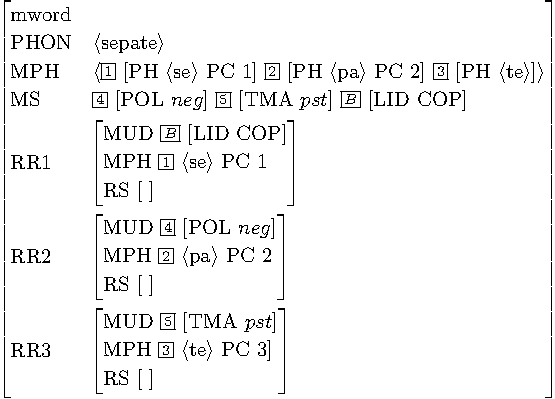
\includegraphics[width=\maxwidth{0.9\textwidth}]{figures/kihm-avm-37.pdf}
\z


\newpage 
This rule should be contrasted with the rule accounting for the ``normal''
order \mbox{/pa te V/} of, e.g., \emph{pa te chante} `didn't sing':


\ea\label{ex:Kihm:38} 
\begin{avm}
\[	\asort{mword}
	phon & $\langle\textrm{patechante}\rangle$\\
	mph & \< \@1 \[ph & $\langle\textrm{pa}\rangle$\\ pc & $1$\],
			 \@2 \[ph & $\langle\textrm{te}\rangle$\\ pc & $2$\],
			 \@3 \[ph & $\langle\textrm{chante}\rangle$\\ pc & $3$\]\>\\
	ms & \< \@{4} [pol~{\itval neg}], \@5 [tma~{\itval pst}], \@{C} [lid~{\itval chante}]\>\\
	rr1 & \[mud & \scval \@{4} [pol~{\itval neg}]\\
			mph & \@1 \[ph & $\langle\textrm{pa}\rangle$\\ pc & $1$\]\\
			rs & \scval [~]
		  \]\\
	rr32& \[mud & \@5 \scval [tma~{\itval pst}]\\
			mph & \@2 \[ph & $\langle\textrm{te}\rangle$\\ pc & $2$\]\\
			rs & \scval [~]
		  \]\\
	rr1 & \[mud & \scval \@{C} [lid~{\itval chante}]\\
			mph & \@3 \[ph & $\langle\textrm{chante}\rangle$\\ pc & $3$\]\\
			rs & \scval [~]
		  \]
\]
\end{avm}
%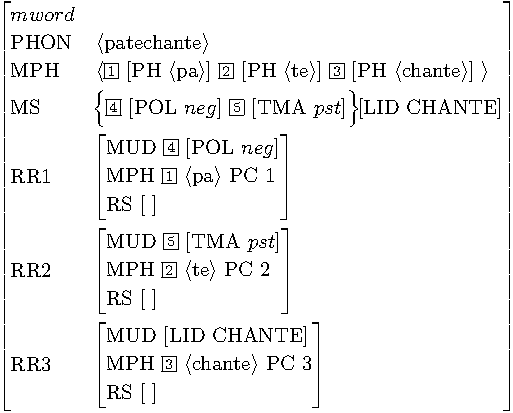
\includegraphics[width=\maxwidth{0.9\textwidth}]{figures/kihm-avm-38.pdf}
\z


The main difference --- apart from the fact that \emph{chante}, like all
verbs but \emph{se} and raising verbs (see above), does not accept null
subjects --- lies in the respective position classes. It is particularly
noteworthy that the mutual ordering of the negator and the TMA marker\is{inflection!marker} is
fixed: $\textit{pa} \prec \text{TMA}$. It is this sequence that appears as a block on
the ``wrong'' side when the verb is \emph{se}.

Examples (\ref{ex:Kihm:6}) \emph{Se frè mwen Jan ye} `It's my brother that John is'
and (\ref{ex:Kihm:14}) \emph{kijan lavi te ye} `how was life' suffice to illustrate
the third stem's environment: its subject must be an NP and its
complement a gap related to clefting as in (\ref{ex:Kihm:6}) or questioning as in
(\ref{ex:Kihm:14}). Hence the following lexical entry:


\ea\label{ex:Kihm:39} 

\begin{avm}
\[	\asort{verb word}
	lid & \@{C} cop\\
	phon & $\langle\textrm{ye}\rangle$\\
	syn & \[	head & \scval [pred~$+$]\\
				val & \[	spr & \@1 \scval \< NP \>\\
							comps & \@2 \scval \<  {\itval gap}\>\\
							arg-st & \scval\@1+\@2
						\]
			\]\\
%	form & \[ stem & $\langle\@{A},\@{B},\@{C}\rangle$\]\\
	sem &	\[	mode & prop\\
				index & s\\
				restr & \[	rln & cop\\
							sit & s\\
							sbj & i\\
							pred & j pred
						\]
			\]
\]
\end{avm}

%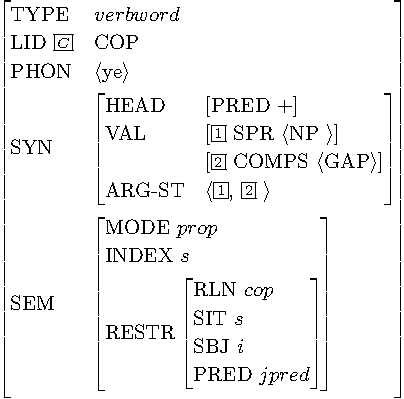
\includegraphics[width=\maxwidth{0.9\textwidth}]{figures/kihm-avm-39.pdf}
\z


As mentioned above, \emph{ye} is neutral as to whether the predicated
property is a stage- or individual-level one. Its occurrance in just one
environment justifies my ranking it as the most non-default stem. On the
other hand, the mutual ranking of the null stem and \emph{se} in terms
of defaultness may be judged moot. The numbers of triggering contexts
are the same, and I can't see any good reason why stage-level\is{stage-level predicate} properties
should be deemed more default than individual-level\is{individual-level predicate} properties. Be it as
it may, since stems must be tagged in any event and nothing much hangs
on the relative ordering of \emph{se} and the null stem, I maintain the
ranking of (\ref{ex:Kihm:28}).

\section{Conclusion: What has been done and what remains to do}

Haitian Creole facts lie precisely at the interface of morphology and
syntax, and it has been the aim of the present article to show how a
word-based morphological model is especially fit to do justice to such
an inherently morphosyntactic character.

Formalizing the data as I just have done is a necessary step in
understanding how things work. It doesn't tell us, however, why things
work the way they do, it doesn't explain why things are as they are.
Explanation in the real sense of the term has to come from outside
formal grammar. In the case at hand, the likeliest source is diachrony,
that is the sociolinguistic conditions under which Haitian Creole
emerged and the nature of the linguistic input at the origin of this
emergence.

As to the first point, our best hypothesis is that Haitian Creole
emerged between the 1680's and the end of the 18\textsuperscript{th}
century as a consequence of the massive importation of African slaves
into Haiti, officially a French possession from 1697 to 1804 %
(see %
%Holm 1989
\citealt{Holm89}%
%
:382--387; %
%Faraclas et al. 2007
\citealt{FaraclasWalicekEtAl2007}%
%
),
%\citep[see][382-387; Faraclas et al. 2007]{Holm89}%
%Holm
%
and that it was mainly the product
of a process of second language acquisition\is{language acquisition!second language acquisition} (SLA) by adults in adverse
conditions, where the target language French\il{French} could only be acquired in
an unguided fashion, ``on the job'', and was not actually acquired, but
only a basic variety of it %
%(Klein \& Perdue 1997)
\citep{Klein1997b}, %
%Klein-Perdue
%
which later expanded
into a full-fledged language. The Africans' knowledge of their first
languages (the substrate) played a role in this process, although
apparently no direct one in the copula issue.

Where it may have proved influential is in the fact that the stage- vs.
individual-level\is{individual-level predicate} contrast is active in what seems to have been Haitian
Creole's main substrate language, namely \ili{Fongbe} %
%(Lefebvre 1998)
\citep{Lefebvre98}%
%Lefebvre
%
. In
\ili{Fongbe} according to %
%Ndayiragidje (1993:63) 
\citet[63]{Ndayiragidje93} %
%Ndayiragidje
%
``only predicates whose
argument structure includes an event position --- \emph{Stage-Level
Predicates}\ldots{} may be clefted, contrary to those that do not
include that position --- \emph{Individual-Level Predicates}'' (my
translation). This is what makes the difference between e.g. \emph{gbà}
`to destroy' and \emph{sè} `to know'. In Haitian Creole as well the same
difference obtains between \emph{kraze} `to destroy' and \emph{konnen}
`to know' so that (\ref{ex:Kihm:40}) is grammatical, whereas (\ref{ex:Kihm:41}) --- possibly meaning
`John does know that language' --- is not %
(%
%Lefebvre 1990 
\citealt{Lefebvre90} %
%
 --- and see (\ref{ex:Kihm:8})--(\ref{ex:Kihm:9})%
%\citep[ --- and see {[}8{]}-{[}9{]}]{Lefebvre90}%
%Lefebvre
%
:

\ea[]{\label{ex:Kihm:40} \gll Se kraze Bouki kraze kay la\\
\textsc{cop} destroy B. destroy house \textsc{def}\\
\glt \trad{What Bouki did to the house was destroy it.}}

\ex[*]{\label{ex:Kihm:41} \gll  Se konnen Jan konnen lang sa a.\\
\textsc{cop} know J. know language \textsc{dem} \textsc{def}\\
\glt Intended: \trad{John does know that language.}}
\z

The \emph{se} vs. null form contrast therefore appears to be a special
case of this overarching contrast permeating the whole verbal lexicon,
which seems to be more central in \ili{Fongbe} than it is in French\il{French}, though it
is present in the latter as well.

Concerning the French\il{French} input, on the other hand, we unsurprisingly hold
no recording of the sort of 17\textsuperscript{th} century French\il{French!17\textsuperscript{th} century French} in
which the arriving slaves were addressed or could pick up from the
native French speakers they were in generally unpleasant contact with.
That it was a colonial koinè\is{colonial koinè} not too different from the central Parisian
dialect, we can be reasonably sure of %
%(Chaudenson 2003)
\citep{Chaudenson2004}% 2003 dans l'original, 2004 dans la bib
%?Chaudenson
%
. Whether it was
the full language or a foreigner talk\is{foreigner talk} reduction of it, we don't know,
though there is evidence that the full lexifier languages were used in
the Caribbean plantations where creole\il{Creole} languages emerged %
%(Alleyne 1980)
\citep{Alleyne1980}%
%Alleyne
%
.

What we can and must do then, is first try to account for the facts that
have been pushed under the rug in the present work, in particular the
strange behaviour of \emph{se} according to whether it is or is not
modified by TMA markers\is{inflection!marker} and/or the negation, and why is then the stage-
vs. individual-level\is{individual-level predicate} contrast neutralized. Secondly, we should look up
17\textsuperscript{th} century French\il{French!17\textsuperscript{th} century French} grammar, using such ressources as
%
%Haase (1935)
\citet{Haase1935a}%
%Haase
%
, in order to determine as much as possible to what extent
the Haitian Creole system inherits from its lexifier's system. For
instance, although the substrate is likely to have been influential as
suggested above, there probably is a relation between the distribution
of \emph{se} and the null stem --- requiring individual and stage-level\is{stage-level predicate}
complements respectively --- and the distribution of \emph{c'est} and
\emph{il/elle est} preceding a nominal complement in
17\textsuperscript{th} century\il{French!17\textsuperscript{th} century French} as well as contemporary French\il{French} %
%(Kupferman
%1979; Boone 1983; Zribi-Hertz to appear)
\citep{Kupferman79,Boone1987,Zribi-Hertz18}%
%Kupferman;?Boone
%
. All this, however, belongs to
the to-do tray. Let's hope it won't linger there too long.


%%% Que faire de cette référence, ce n'est pas un titre de Robert Damoiseau mais de Anne Fauchois !?
%Damoiseau, Robert (1985). \emph{Nature et fonction des monèmes `se' en
%    créole haïtien}. Port-au-Prince: Centre de Linguistique, Université
%d'Etat d'Haïti.
%
%\nocite{Alleyne1980}
%\nocite{Bender2000}
%\nocite{Blevins06}
%\nocite{Blevins14}
%\nocite{bonami2015}
%\nocite{Booij96}
%\nocite{Boone1987}
%\nocite{Carlson1977}
%\nocite{ChalmersKenolEtAl2015}
%\nocite{Chaudenson2004}
%%\nocite{Chierchia1999}
%\nocite{ZwickyKaisseEtAl1987}
%\nocite{Crysmann2015}
%\nocite{Damoiseau1996}
%\nocite{Degraff1992}
%\nocite{DeGraff2007}
%\nocite{Deprez1992}
%\nocite{Deprez1992a}
%\nocite{DeprezVinet1997}
%\nocite{Diesing1988}
%\nocite{FaraclasWalicekEtAl2007}
%\nocite{Fattier2013}
%\nocite{Glaude2012}
%\nocite{Haase1935a}
%\nocite{Hayes1990}
%\nocite{Higgins79}
%\nocite{Holm89}
%\nocite{Huddleston2002}
%\nocite{Kihm93}
%\nocite{Kihm03}
%\nocite{Klein1997b}
%\nocite{Kratzer1995}
%\nocite{Kupferman79}
%\nocite{Lefebvre90}
%\nocite{Lefebvre98}
%\nocite{Lyons99}
%\nocite{Maiden11}
%\nocite{Mateus89}
%\nocite{Matthews72}
%\nocite{Ndayiragidje93}
%\nocite{Pompilius76}
%\nocite{Sag12:\is{}
%\nocite{Sag03}
%\nocite{Sag99}
%\nocite{Stump01}
%\nocite{Tessonneau80}
%\nocite{Valdman78}
%\nocite{Valdman81}
%\nocite{VanEynde1994}
%\nocite{Zribi-Hertz18}
%\nocite{Zwicky85b}
%\nocite{Zwicky90}

\is{copula|)}
\il{French-based creole!Haitian Creole|)}

{\sloppy
\printbibliography[heading=subbibliography,notkeyword=this]
}

\end{document}
